%
% Copyright 2018 Joel Feldman, Andrew Rechnitzer and Elyse Yeager.
% This work is licensed under a Creative Commons Attribution-NonCommercial-ShareAlike 4.0 International License.
% https://creativecommons.org/licenses/by-nc-sa/4.0/
%
\questionheader{ex:s2.1}
%%%%%%%%%%%%%%%%%%
\subsection*{\Conceptual}
%%%%%%%%%%%%%%%%%%
\begin{question} Shown below is the graph $y=f(x)$. If we choose a point $Q$ on the graph to the \emph{left} of the $y$-axis, is the slope of the secant line through $P$ and $Q$ positive or negative?
If we choose a point $Q$ on the graph to the \emph{right} of the $y$-axis, is the slope of the secant line through $P$ and $Q$ positive or negative?
\begin{center}
\begin{tikzpicture}
\YEaaxis{5}{5}{1}{4}
\draw[thick] plot[domain=-5:-.25] (\x+.25,{-3/(\x-.6)});
\draw[thick] plot[domain=.25:5] (\x-.25,{3/(\x+.6)}) node[above]{$y=f(x)$};
\draw (0,60/17) node[vertex, label=right:$P$]{};
\end{tikzpicture}
\end{center}
\end{question}
\begin{answer} If $Q$ is to the left of the $y$ axis, the secant line has positive slope;
if $Q$ is to the right of the $y$ axis, the secant line has negative slope.
\end{answer}
\begin{solution} If $Q$ is to the left of the $y$ axis, the line through $Q$ and $P$ is increasing, so the secant line has positive slope.
If $Q$ is to the right of the $y$ axis, the line through $Q$ and $P$ is decreasing, so the secant line has negative slope.
\end{solution}

\begin{Mquestion} Shown below is the graph $y=f(x)$.
\begin{enumerate}[(a)]
\item\label{s2.1p2.1} If we want the slope of the secant line through $P$ and $Q$ to \emph{increase}, should we slide $Q$ closer to $P$, or further away?
\item\label{s2.1p2.2} Which is larger, the slope of the tangent line at $P$, or the slope of the secant line through $P$ and $Q$?
\end{enumerate}
\begin{center}
\begin{tikzpicture}
\YEaxis{4}{3}
\draw[thick] plot[domain=-3.5:3.5](\x,{(\x+4)*(\x+4)/10-2.5});
\draw (3.25,2.76) node[vertex, label=right:$P$]{};
\draw (-1,-1.6) node[vertex, label=below right:$Q$]{};
\end{tikzpicture}
\end{center}
\end{Mquestion}
\begin{hint} You can use \eqref{s2.1p2.1} to explain \eqref{s2.1p2.2}.
\end{hint}
\begin{answer}\eqref{s2.1p2.1} closer \qquad
\eqref{s2.1p2.2} the tangent line has the larger slope
\end{answer}
\begin{solution}\eqref{s2.1p2.1} By drawing a few pictures, it's easy to see that sliding $Q$ closer to $P$, the slope of the secant line increases.

\eqref{s2.1p2.2} Since the slope of the secant line increases the closer $Q$ gets to $P$, that means the tangent line (which is the limit as $Q$ approaches $P$) has a larger slope than the secant line between $Q$ and $P$ (using the location where $Q$ is right now).

Alternately, by simply sketching the tangent line at $P$, we can see that has a steeper slope than the secant line between $P$ and $Q$.
\end{solution}

\begin{question} Group the functions below into collections whose secant lines from $x=-2$ to $x=2$ all have the same slopes.
\begin{center}
\begin{tikzpicture}
\YEaxis{2.25}{1.5}
\draw[thin, gray, dotted] (-2,-1.5) grid (2,1.5);
\draw (-2,.2)--(-2,-.2) node[below]{$-2$};
\draw (2,.2)--(2,-.2) node[below]{$2$};
\draw[thick] (-2,-1)--(2,0);
\draw (0,-2) node{(a)};
\end{tikzpicture}\hfill
\begin{tikzpicture}
\YEaxis{2.25}{1.5}
\draw[thin, gray, dotted] (-2,-1.5) grid (2,1.5);
\draw (-2,.2)--(-2,-.2) node[below]{$-2$};
\draw (2,.2)--(2,-.2) node[below]{$2$};
\draw[thick] (-2,1.5)--(2,0.5);
\draw (0,-2) node{(b)};
\end{tikzpicture}\hfill
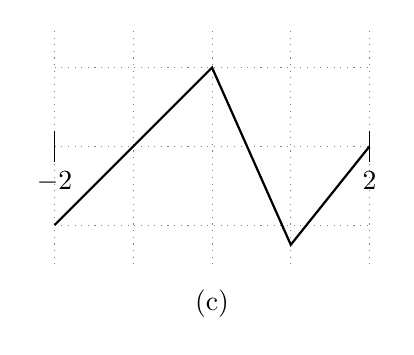
\begin{tikzpicture}
\YEaxis{2.25}{1.5}
\draw[thin, gray, dotted] (-2,-1.5) grid (2,1.5);
\draw (-2,.2)--(-2,-.2) node[below]{$-2$};
\draw (2,.2)--(2,-.2) node[below]{$2$};
\draw[thick] (-2,-1)--(0,1)--(1,-1.25)--(2,0);
\draw (0,-2) node{(c)};
\end{tikzpicture}
\end{center}
%
\begin{center}
\begin{tikzpicture}
\YEaxis{2.25}{1.5}
\draw[thin, gray, dotted] (-2,-1.5) grid (2,1.5);
\draw (-2,.2)--(-2,-.2) node[below]{$-2$};
\draw (2,.2)--(2,-.2) node[below]{$2$};
\draw[thick] (-2,1)--(2,1);
\draw (0,-2) node{(d)};
\end{tikzpicture}\hfill
\begin{tikzpicture}
\YEaxis{2.25}{1.5}
\draw[thin, gray, dotted] (-2,-1.5) grid (2,1.5);
\draw (-2,.2)--(-2,-.2) node[below]{$-2$};
\draw (2,.2)--(2,-.2) node[below]{$2$};
\draw[thick] (-2,0)--(2,1);
\draw (0,-2) node{(e)};
\end{tikzpicture}\hfill
\begin{tikzpicture}
\YEaxis{2.25}{1.5}
\draw[thin, gray, dotted] (-2,-1.5) grid (2,1.5);
\draw (-2,.2)--(-2,-.2) node[below]{$-2$};
\draw (2,.2)--(2,-.2) node[below]{$2$};
\draw[thick] (-2,1)--(-1,-1)--(1,-1)--(2,0);
\draw (0,-2) node{(f)};
\end{tikzpicture}
\end{center}
\end{question}
\begin{hint} Your calculations for slope of the secant lines will all have the same denominators; to save yourself some time, you can focus on the numerators.
\end{hint}
\begin{answer} \{(a), (c), (e)\}, \quad\{(b),(f)\},\quad \{(d)\}
\end{answer}
\begin{solution} The slope of the secant line will be $\dfrac{f(2)-f(-2)}{2-(-2)} = \dfrac{f(2)-f(-2)}{4}$, in every part. So, if two lines have the same slope, that means their differences $f(2)-f(-2)$ will be the same.

The graphs in (a),(c), and (e) all have $f(2)-f(-2)=1$, so they all have the same secant line slope. The graphs in (b) and (f) both have $f(2)-f(-2)=-1$, so they both have the same secant line slope. The graph in (d) has $f(2)-f(-2)=0$, and it is the only graph with this property, so it does not share its secant line slope with any of the other graphs.
\end{solution}


%%%%%%%%%%%%%%%%%%
\subsection*{\Procedural}
%%%%%%%%%%%%%%%%%%


\begin{question}
Give your best approximation of the slope of the tangent line to
the graph below at the point $x=5$.
\begin{center}
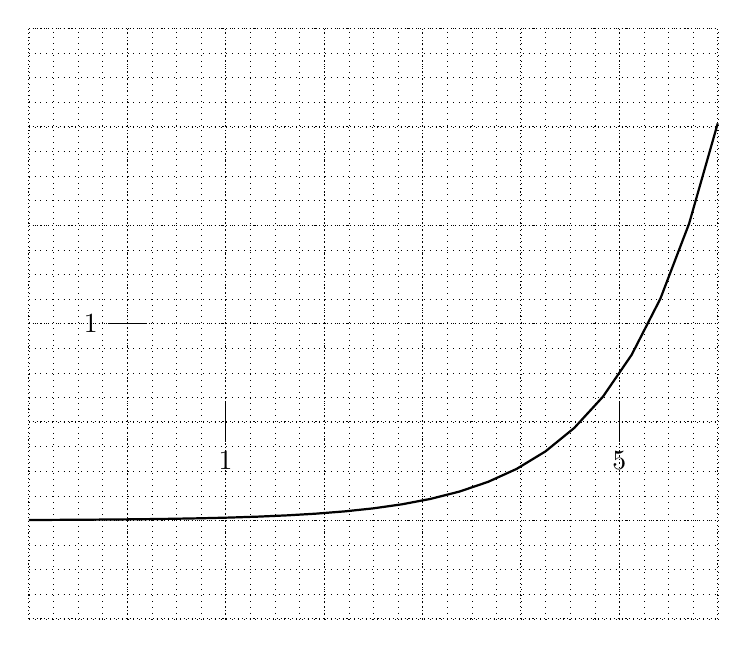
\begin{tikzpicture}[scale=1.25]
\YEaaxis{1.1}{6.1}{2.1}{4.1}
\draw[densely dotted] (-1,-2) grid (6,4);
\draw (1,.2)--(1,-.2) node[below]{1};
\draw (5,.2)--(5,-.2) node[below]{5};
\draw (.2,1)--(-.2,1) node[left]{1};
\draw[dotted, ultra thin] (-1,-2) grid[step=.25] (6,4);
\draw[thick] plot[domain=-1:6](\x,{exp(\x)/100-1});
\end{tikzpicture}
\end{center}
\end{question}
\begin{hint} You can do this by calculating several secant lines. You can also do this by getting out a ruler and trying to draw the tangent line very carefully.
\end{hint}
\begin{answer} Something like $1.5$. A reasonable answer would be between 1 and 2.
\end{answer}
\begin{solution} A good approximation from the graph is $f(5)=0.5$. We want to find a secant line whose endpoints are both very close to $x=5$, but that also give us clear $y$-values. It looks like $f(5.25) \approx 1$, and $f(4.75)\approx \frac{1}{8}$. The secant line from $x=5$ to $x=5.25$ has approximate slope $\dfrac{f(5.25)-f(5)}{5.25-5}\approx \dfrac{1-.5}{.25}=2$. The secant line from $x=5$ to $x=4.75$ has approximate slope $\dfrac{0.5-\frac{1}{8}}{5-4.75}=\dfrac{3}{2}$.

The graph increases more and more quickly (gets steeper and steeper), so it makes sense that the secant line to the left of $x=5$ has a smaller slope than the secant line to the right of $x=5$.  Also, if you're taking secant lines that have endpoints farther out from $x=5$, you'll notice that the slopes of the secant lines change quite dramatically. You have to be very, very close to $x=5$ to get any kind of accuracy.

If we split the difference, we might approximate the slope of the secant line to be the average of $\frac{3}{2}$ and $2$, which is $\frac{7}{4}$.

Another way to try to figure out the tangent line is by carefully drawing it in with a ruler. This is shown here in blue:
\begin{center}
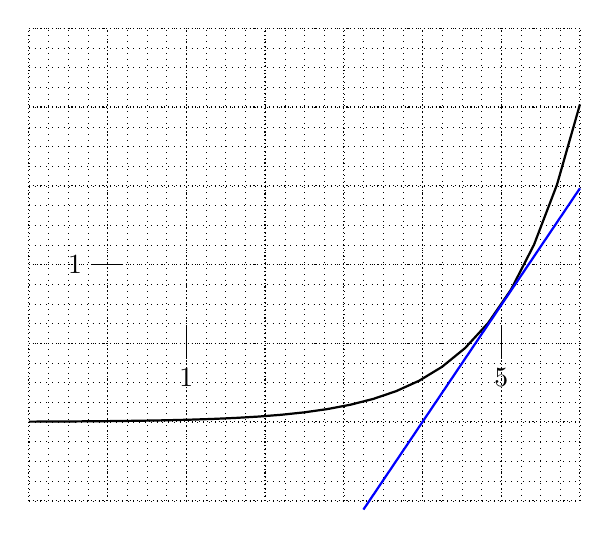
\begin{tikzpicture}
\YEaaxis{1.1}{6.1}{2.1}{4.1}
\draw[densely dotted] (-1,-2) grid (6,4);
\draw (1,.2)--(1,-.2) node[below]{1};
\draw (5,.2)--(5,-.2) node[below]{5};
\draw (.2,1)--(-.2,1) node[left]{1};
\draw[dotted, ultra thin] (-1,-2) grid[step=.25] (6,4);
\draw[thick] plot[domain=-1:6](\x,{exp(\x)/100-1});
\draw[thick, blue] plot[domain=3.25:6](\x,{1.484*(\x-5)+.484});
\end{tikzpicture}
\end{center}
It's much easier to take the slope of a line than a curve, and this one looks like it has slope about 1.5. However, we drew this with a computer: by hand it's much harder to draw an accurate tangent line. (That's why we need calculus!)

The actual slope of the tangent line to the function at $x=5$ is about $1.484$. This is extremely hard to figure out just from the graph--by hand, a guess between $1.25$ and $1.75$ would be very accurate.
\end{solution}


\begin{Mquestion}On the graph below, sketch the tangent line to $y=f(x)$ at $P$. Then, find two points $Q$ and $R$  on the graph so that the secant line through $Q$ and $R$ has the same slope as the tangent line at $P$.
\begin{center}
\begin{tikzpicture}
\YEaxis{5}{3}
\draw[thick] plot[domain=0:4.5](\x,{\x*\x/4-2}) node[below right]{$y=f(x)$};
\draw[thick] (-4.5,0) cos (-2.25,-1) sin (0,-2);
\draw (1,-7/4) node[vertex, label=below:$P$]{};
\end{tikzpicture}
\end{center}
\end{Mquestion}
\begin{hint} There are many possible values for $Q$ and $R$.
\end{hint}
\begin{answer} There is only one tangent line to $f(x)$ at $P$ (shown in blue), but there are infinitely many choices of $Q$ and $R$ (one possibility shown in red).
\begin{center}
\begin{tikzpicture}
\YEaxis{5}{3}
\draw[thick] plot[domain=0:4.5](\x,{\x*\x/4-2}) node[below right]{$y=f(x)$};
\draw[thick] (-4.5,0) cos (-2.25,-1) sin (0,-2);
\draw (1,-7/4) node[vertex, label=below:$P$]{};
\draw[blue, thick] (-1,-11/4)--(4,-1/4);
\draw[red] (0,-2) node[vertex, label=above left:$Q$]{};
\draw[red] (2,-1) node[vertex, label=above:$R$]{};
\draw[red, thick] (-1,-2.5)--(4,0);
\end{tikzpicture}
\end{center}
\end{answer}
\begin{solution} There is only one tangent line to $f(x)$ at $P$ (shown in blue), but there are infinitely many choices of $Q$ and $R$ (one possibility shown in red).
One easy way to sketch the secant line on paper is to draw any line parallel to the tangent line, and choose two intercepts with $y=f(x)$.
\begin{center}
\begin{tikzpicture}
\YEaxis{5}{3}
\draw[thick] plot[domain=0:4.5](\x,{\x*\x/4-2}) node[below right]{$y=f(x)$};
\draw[thick] (-4.5,0) cos (-2.25,-1) sin (0,-2);
\draw (1,-7/4) node[vertex, label=below:$P$]{};
\draw[blue, thick] (-1,-11/4)--(4,-1/4);
\draw[red] (0,-2) node[vertex, label=above left:$Q$]{};
\draw[red] (2,-1) node[vertex, label=above:$R$]{};
\draw[red, thick] (-1,-2.5)--(4,0);
\end{tikzpicture}
\end{center}
\end{solution}


\begin{Mquestion}Mark the points where the curve shown below has a tangent line with slope $0$.
\begin{center}
\begin{tikzpicture}
\YEaxis{5}{3}
\draw[thick] plot[domain=2:4.5](\x,{-(\x-3)*(\x-3)/2-1/2}) node[below right]{$y=f(x)$};
\draw[thick] plot[domain=-1:2](\x,{\x*\x/4-2});
\draw[thick] plot[smooth] coordinates{(-5,3) (-4,1.3) (-3,1) (-2,-1) (-1,-7/4)};
\end{tikzpicture}\end{center}
(Later on, we'll learn how these points tell us a lot about the shape of a graph.)
\end{Mquestion}
\begin{hint} A line with slope $0$ is horizontal.
\end{hint}
\begin{answer}
\begin{center}
\begin{tikzpicture}
\YEaxis{5}{3}
\draw[thick] plot[domain=2:4.5](\x,{-(\x-3)*(\x-3)/2-1/2}) node[below right]{$y=f(x)$};
\draw[thick] plot[domain=-1:2](\x,{\x*\x/4-2});
\draw[thick] plot[smooth] coordinates{(-5,3) (-4,1.3) (-3,1) (-2,-1) (-1,-7/4)};
\draw[blue] (-3.5,1.15) node[vertex]{};
\draw[blue] (0,-2) node[vertex]{};
\draw[blue] (3,-1/2) node[vertex]{};
\end{tikzpicture}\end{center}
\end{answer}
\begin{solution}
Any place the graph looks flat (if you imagine zooming in) is where the tangent line has slope 0. This occurs three times.
\begin{center}
\begin{tikzpicture}
\YEaxis{5}{3}
\draw[thick] plot[domain=2:4.5](\x,{-(\x-3)*(\x-3)/2-1/2}) node[below right]{$y=f(x)$};
\draw[thick] plot[domain=-1:2](\x,{\x*\x/4-2});
\draw[thick] plot[smooth] coordinates{(-5,3) (-4,1.3) (-3,1) (-2,-1) (-1,-7/4)};
\draw[blue] (-3.5,1.15) node[vertex]{};
\draw[blue] (0,-2) node[vertex]{};
\draw[blue] (3,-1/2) node[vertex]{};
\end{tikzpicture}\end{center}
Notice that two of the indicated points are at a low point and a high point, respectively. Later, we'll use these places where the tangent line has slope zero to find where a graph achieves its biggest and smallest values.
\end{solution}
